\chapter{LIERATURE SURVEY}

\section*{Paper-based Document Authentication using Digital Signature and QR Code
}

\textit{by Maykin Warasart, Pramote Kuacharoen
Department of Computer Science, Graduate School of Applied Statistics
National Institute of Development Administration
Published : ICCET 2012
}\cite{paper_based_document_authentication}\\

\noindent{
    There are still needs for paper-based documents in certain circumstances where electronic documents cannot efficiently replace them. For example, documents issued by the government such as birth certificates, driver licenses, and passports must be paper-based. With advanced scanning and printing technologies, paper-based document fraud can easily be conducted without significant high cost.\\

In this paper, an implementation of paper-based document authentication is presented. The integrity of the text message and the author of the document can be verified with the use of a digital signature and QR code. The proposed method can be automatic or semi-automatic. It is semi-automatic when the OCR is not accurate and it requires the user to visually compare the text message on the paper and the one obtained from the QR code. However, this method does provide convenience for the user in dealing with a large amount of documents.\\


	Model architecture 
    }Senders Process

    \begin{figure}[H]
        \centering
        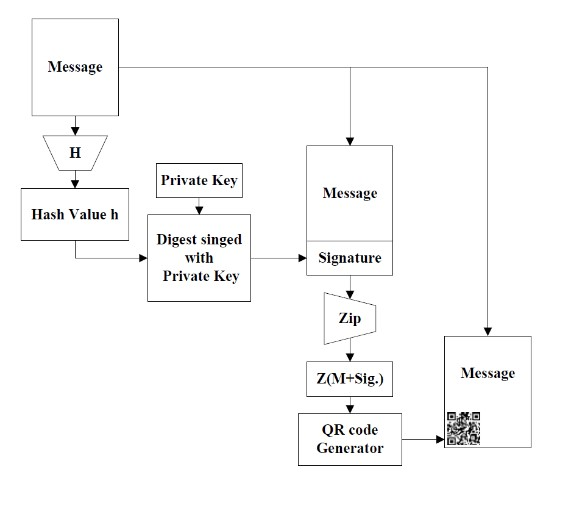
\includegraphics[width=\textwidth]{imgs/figure_2.1.1.jpg}
        \caption{Sender Process of Paper-based Document Authentication using Digital Signature and QR Code }
        \label{fig:Receiver Process of Paper-based Document Authentication using Digital Signature and QR Code}
        \end{figure}

\noindent{
    For this process, the message and the corresponding verification code in a form of QR code are printed on paper. After the message is composed, its hash value is generated. Then, the hash value h is encrypted with the private key of a sender resulting in the digital signature on the message M. After that, the message M and the digital signature are combined and compressed to reduce size so that they can be stored in a QR code. The compressed message and signature are fed into a QR code generator. After the QR code has been created, message M together with the QR code are printed on to paper and sent to a receiver. The simplified
process of sender is shown in Figure 2.1 \\
}
Receiver process
\begin{figure}[H]
    \centering
    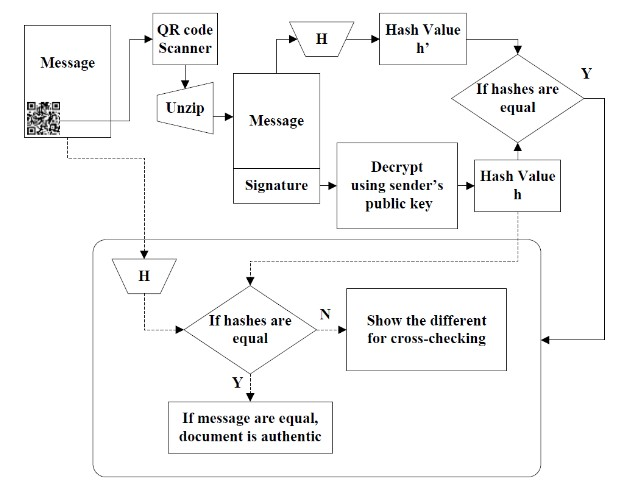
\includegraphics[width=\textwidth]{imgs/figure_2.1.2.jpg}
    \caption{Receiver Process of Paper-based Document Authentication using Digital Signature and QR Code }
    \label{fig:Receiver Process of Paper-based Document Authentication using Digital Signature and QR Code}
    \end{figure}
\noindent{
    When a receiver obtains the document from a sender, he/she may verify the authenticity of the document by scanning the document and processing the image as illustrated in Figure 2.2. The verification process starts with checking the integrity of the information stored in the QR code. The information in the QR code consists of the message and the signature of the sender on the message, which are compressed. After scanning the QR code and uncompressing the data, the signature can be verified by comparing the hash value of the obtained message and the value from decrypting the signature using the sender’s public key. If both values are identical, the signature is valid. To validate the printed message, the Optical Character Recognition (OCR) must be employed. The hash value of the message obtained from the OCR is computed and compared with the hash value obtained from the message in the QR code. If they are identical, the printed message is authentic. However, if they are different, it cannot be concluded that the printed message has been modified. Further human review must be conducted. This is because the OCR may not be 100\% accurate. The message obtained from the QR code can be shown next to the printed message which can be visually inspected. \\
}
\vspace{1cm}



\noindent{\underline{CONCLUSION:}
Authenticity of paper-based documents can be achieved by using digital signatures and QR codes without accessing the database. The verification process can be done automatically if the OCR is accurate. Otherwise, human inspection is required. Even with this semi-automatic process, this proposed method facilitates the verification process. The inspector can see the differences between the printed message and the message in the QR code.\\
}

\section*{Towards a framework of A Secure E-Qualification Certificate System}

\textit{~ Lisha Chen-Wilson, Dr David Argles
School of Electronic and Computer Science
University of Southampton, United Kingdom
Published: 2010 Second International Conference on Computer Modeling and Simulation
}\cite{e-qualification_certificate_system}\\

\noindent{The paper-based certificates also  come with management problems. They are easily lost or  damaged, and they are hard to prove genuine when Presented. The field of e-Learning provides technological developments, such as e-portfolios, which are being explored as an improvement over paper-based portfolios in the job and course application process. However, forged certificates exist due to poor security in e-portfolio systems. Therefore, the students’ claimed achievements within e-portfolios need to be verified.\\

In order to solve the above problems, it is necessary to implement an electronic version of qualification certificates (e-certificate) that are at least as valid as the paper-based certificates, and can be used either as a standalone application or fitted within other applications, such as eportfolios. It needs to be easy to use and suit all levels of students while including high security methods to prevent forgery. The students need to have control over the usage of such e-certificate, and there must also be a verification method provided. We need to secure the e-certificate system, not just the e-certificate.\\
}

\begin{figure}[H]
    \centering
    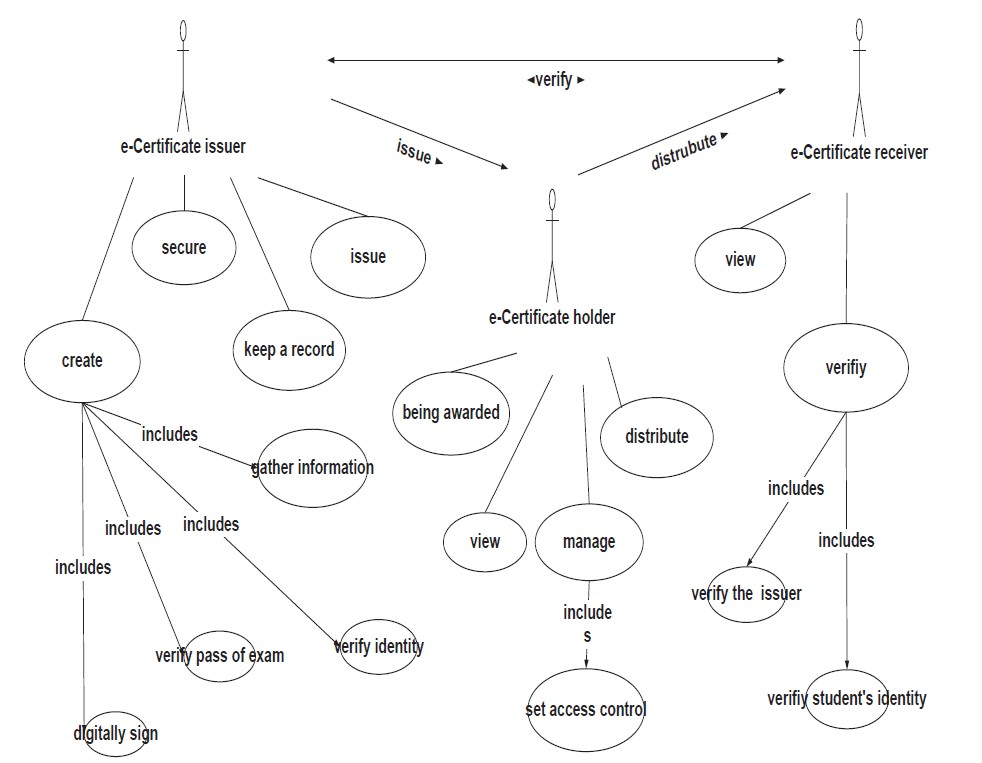
\includegraphics[width=\textwidth]{imgs/figure_2.2.1.jpg}
    \caption{Management of secure E-Qualification Certificate System
    }
    \label{fig:Management of secure E-Qualification Certificate System}
    \end{figure}

\noindent{An e-certificate issuer is a body that creates and issues the certificate, such as a college or a university. They may:}

\begin{itemize}
    \item Issue a huge range and amount of certificates

    \item Restrict database access control for any in coming verification request to minimize database attacks
  \end{itemize}

  \noindent{An e-certificate owner is the certificate holder who has successfully passed the qualification certification process and gained the award, such as a student or a graduate.
  An e-certificate reviewer is a body or a person who receives the certificate in support of an application. This may be an academic institution or an employer. They:
    }
    \begin{itemize}
        \item could be an individual or big organizations
        \item may receive e-qualification certificates as part of applications or within e-portfolios
\item may have few IT skills or may have a team of IT literate staff with high tech IT equipments
\item may need to check a few qualifications occasionally or may need to check a huge amount of qualifications efficiently
      \end{itemize}
    
\section*{Bitcoin: A Peer-to-Peer Electronic Cash System
}

\textit{by Satoshi Nakamoto }\cite{bitcoin_paper}\\

\noindent{
    In this paper the author introduces a  purely peer-to-peer version of electronic cash that would allow online payments to be sent directly from one party to another without going through a financial institution. Digital signatures provide part of the solution, but the main benefits are lost if a trusted third party is still required to prevent double-spending.We propose a solution to the double-spending problem using a peer-to-peer network. The network timestamps transactions by hashing them into an ongoing chain of hash-based proof-of-work, forming a record that cannot be changed without redoing the proof-of-work. The longest chain not only serves as proof of the sequence of events witnessed, but proof that it came from the largest pool of CPU power. As long as a majority of CPU power is controlled by nodes that are not cooperating to attack the network, they'll generate the longest chain and outpace attackers. The network itself requires minimal structure. Messages are broadcast on a best effort basis, and nodes can leave and rejoin the network at will, accepting the longest proof-of-work chain as proof of what happened while they were gone.\\

\underline{Proof of work:}
To implement a distributed timestamp server on a peer-to-peer basis, we will need to use a proof of- work system similar to Adam Back's Hashcash, rather than newspaper or Usenet posts.The proof-of-work involves scanning for a value that when hashed, such as with SHA-256, the hash begins with a number of zero bits. The average work required is exponential in the number of zero bits required and can be verified by executing a single hash.For our timestamp network, we implement the proof-of-work by incrementing a nonce in the block until a value is found that gives the block's hash the required zero bits. Once the CPU effort has been expended to make it satisfy the proof-of-work, the block cannot be changed without redoing the work. As later blocks are chained after it, the work to change the block would include redoing all the blocks after it.\\
}

\begin{figure}[H]
    \centering
    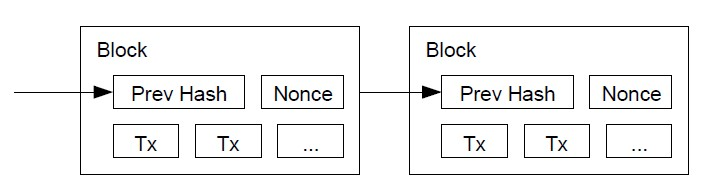
\includegraphics[width=\textwidth]{imgs/figure_2.3.1.jpg}
    \caption{Block representation of Blockchain
    }
    \label{fig:Block representation of Blockchain}
    \end{figure}

\noindent{
    The proof-of-work also solves the problem of determining representation in majority decision making. If the majority were based on one-IP-address-one-vote, it could be subverted by anyone able to allocate many IPs. Proof-of-work is essentially one-CPU-one-vote. The majority decision is represented by the longest chain, which has the greatest proof-of-work effort invested in it. If a majority of CPU power is controlled by honest nodes, the honest chain will grow the fastest and outpace any competing chains. To modify a past block, an attacker would have to redo the proof-of-work of the block and all blocks after it and then catch up with and surpass the work of the honest nodes. We will show later that the probability of a slower attacker catching up diminishes exponentially as subsequent blocks are added.\\
To compensate for increasing hardware speed and varying interest in running nodes over time, the proof-of-work difficulty is determined by a moving average targeting an average number of blocks per hour. If they're generated too fast, the difficulty increases.
}

\section*{ Educational Certificate Verification System Using Blockchain}

\textit{by  Dinesh Kumar K  Senthil P , Manoj Kumar D.S Publish:INTERNATIONAL JOURNAL OF SCIENTIFIC \& TECHNOLOGY RESEARCH VOLUME 9,ISSUE 03, MARCH 2020}\cite{educational_certificate_verification_system_using_blockchain}\\

\noindent{
    The students' achievements available in the form of degree certificate, mark sheet, value added certificate, etc., will become an important weightage for recruitment or higher studies. The Education institution awards and degree certificates may have only the names of the institution and the student’s data. In this scenario there is a lack of effective anti forge mechanism, due to this many times the graduation certificate to be forged often is found. To solve the problem of fake certificates, the blockchain technology would store the certificate in digital form. The immutability nature of blockchain makes digital certificates in the distributed ledger very difficult to tamper or modify. Also, it is very easy to verify the originality of a digital certificate.
}

\begin{figure}[H]
    \centering
    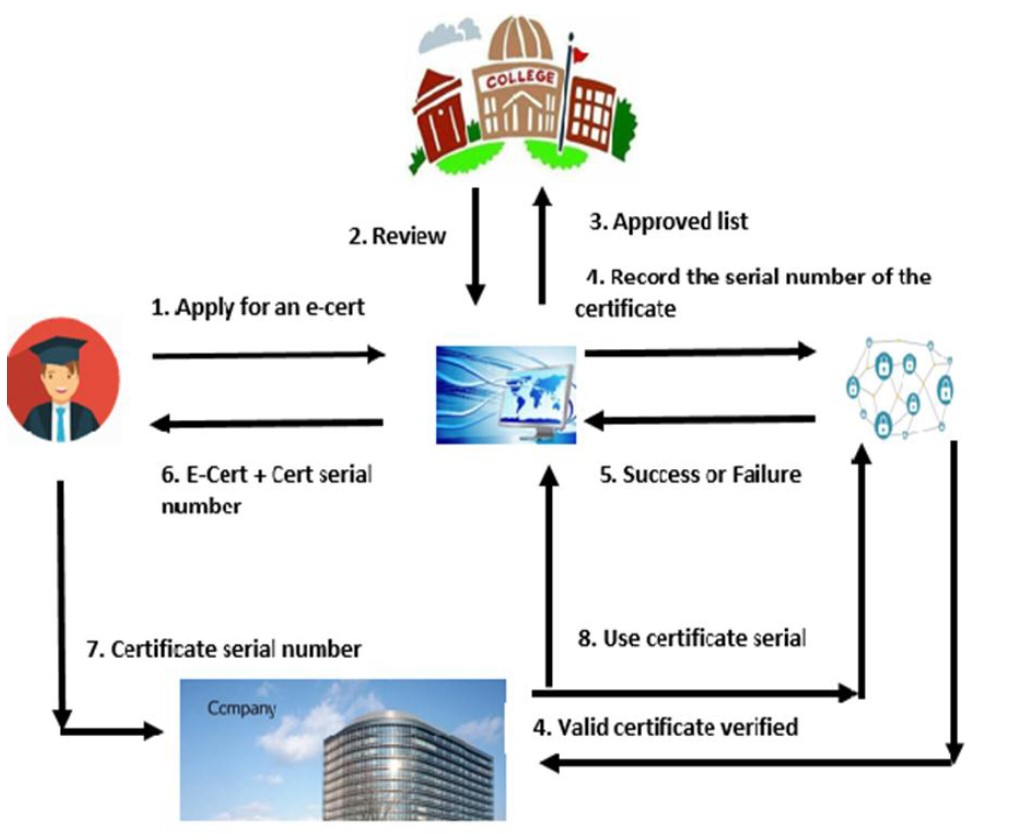
\includegraphics[width=\textwidth]{imgs/figure_2.4.1.jpg}
    \caption{Process of issuing digital certificates
    }
    \label{fig:Process of issuing digital certificates}
    \end{figure}

    \noindent{
The process of issuing digital certificates in the system is as follows. First step, generate the hash value for the certificate using double SHA256. Store the fixed length hash value as a transaction in the block. This transaction is validated by the members in the blockchain, once it is trusted as a valid transaction then the block is added with existing blockchain. Accepting and rejecting will be done using consensus algorithms . The consensus algorithm may be chosen based on number of nodes, and transactions. The system will generate the related QR code and inquiry string code to affix in the hardcopy certificate. The system provides the unit to authenticate the hardcopy certificate through phone scanner or website. The immutability nature of the distributed ledger, the system provides not only verification of certificate and also it stores the certificate in digital form forever\\}

\noindent{\underline{Result:}
Transparency and data immutability are the main features of blockchain application. It is a distributed ledger where nodes in the network validate and make final consensus to add the data in the network. The process of academic certificate generation is open and distributed among the parties where any organization or parties can verify information of any academic certificate using this blockchain system. The Ethereum blockchain also ensures data stored on the blockchain network is encrypted, therefore only the certificate owner can see and share this data as they wish. In conclusion, academic institutions are able to collaborate with other employers and publish credentials on the blockchain to eradicate fake educational certificates}


\section*{IPFS - Content Addressed, Versioned, P2P File System
}

\textit{by Juan Benet}\cite{IPFS}\\

\noindent{
    The InterPlanetary File System (IPFS) is a peer-to-peer distributed le system that seeks to connect all comput- ing devices with the same system of les. In some ways, IPFS is similar to the Web, but IPFS could be seen as a single BitTorrent swarm, exchanging objects within one Git repository. In other words, IPFS provides a high throughput content-addressed block storage model, with content- addressed hyperlinks. This forms a generalized Merkle DAG, a data structure upon which one can build versioned systems, blockchains, and even a Permanent Web. IPFS combines a distributed hash table, an incentivized block ex-change, and a self-certifying namespace. IPFS has no single point of failure, and nodes do not need to trust each other.\\

IPFS is peer-to-peer; no nodes are privileged. IPFS nodes store IPFS objects in local storage. Nodes connect to each other and transfer objects. These objects represent les and other data structures. The IPFS Protocol is divided into a stack of sub-protocols responsible for different functionality:}

\begin{enumerate}
    \item  Identities - manage node identity generation and verification.
    \item Network - manages connections to other peers, uses various underlying network protocols. Configurable.
    \item Routing - maintains information to locate specific peers and objects. Responds to both local and remote queries. Defaults to a DHT, but is swappable.
    \item  Exchange - a novel block exchange protocol (BitSwap) that governs decent block distribution. Modeled as a market, weakly incentivizes data replication. Trade Strategies swappable
\item Objects - a Merkle DAG of content-addressed immutable objects with links. Used to represent arbitrary data structures, e.g. le hierarchies and communication systems.
\item Files - versioned le system hierarchy inspired by Git.
\item Naming - A self-certifying mutable name system.
\end{enumerate}

\section*{IPFS Based Storage Model for Blockchain} 

\textit{by  Qinhong Zeng, Yi Li, Ping Chen, Xinghua Dong
2018 IEEE/WIC/ACM International Conference on Web Intelligence}\cite{ipfsbasedmodelforblockchain}\\

\noindent{
    This paper suggests making use of IPFS to store the certificates on IPFS.
    Take all the transactions of a block put it in a document and upload it on IPFS
    Further take the IPFS link as the transaction to the blockchain.
    This reduces the storage in blocks of blockchain there by reducing the load.
    }
    \begin{figure}[H]
        \centering
        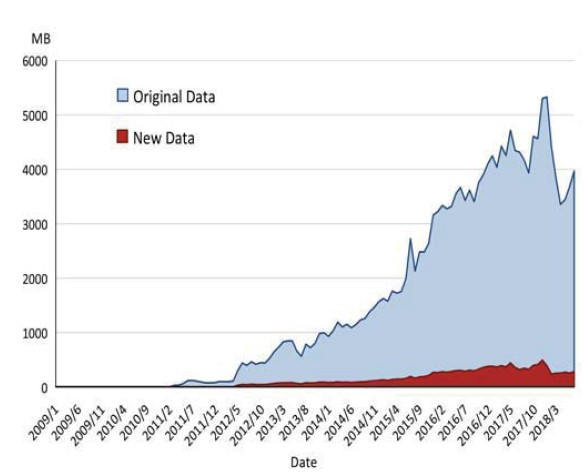
\includegraphics[width=\textwidth]{imgs/figure_2.6.1.jpg}
        \caption{Comparision of the sum of the block data in each before and after data processing
        }
        \label{fig:Comparision of the sum of the block data in each before and after data processing}
        \end{figure}
    \noindent{
       \underline{Results:}
It can be seen from the result that it has a certain degree of improvement in storage space,  security and new node synchronization speed.
}

\section*{Tamper-Proof Certificate Management System} 

\textit{by Raghav, Nitish Andola, Rakhi Verma, S. Venketesan, Shekar Verma
2019 IEEE Conference on Information and Communication Technology
}\cite{tamper_proof_certification}\\

\noindent{
    Certificates are a proof of achievement/membership like University degrees and school certificates etc. Certificates as proof are essential in society but our current certificate management system is mostly analog, inefficient and amenable to forgery . Due to the ineffective anti-forge mechanism, forged certificates are becoming prevalent. To solve this problem, secure certificate management is proposed, then also security problems like privacy, transparency and forgeries still exist. We propose a tamper-proof certificate management using hyperledger which provides a secure anti-forge mechanism. Hyperledger has unmodifiable and other suitable properties of the blockchain that helps to minimize the problem of forgery. We use IPFS (Inter Planetary File System) for storing the certificate. The procedure for issuing the certificates is to first generate the degree of a student using a portal, meanwhile then calculate its hash value and encrypt it using asymmetric encryption. Then store file into
IPFS. Finally, we make a transaction that contains metadata of certificate which stores in the blockchain system. Then, chaincode is used for verification of the user's document. We also reduce the time complexity of searching and verifying the multiple documents of the same user. Our proposed work enhances the credibility of paper-based certificates, and also reduces the risk of forging certificates. We also show the performance of generating transactions in hyperledger.	}
    \begin{figure}[H]
        \centering
        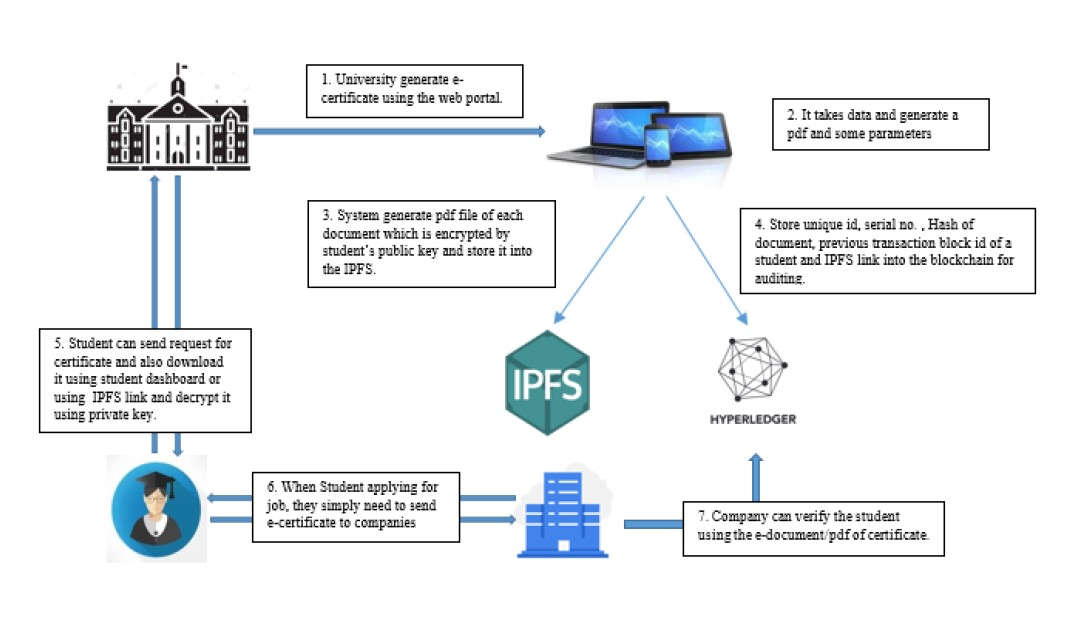
\includegraphics[width=\textwidth]{imgs/figure_2.7.1.jpg}
        \caption{Generating certificates using IPFS and hyperledger}
        \label{fig:Generating certificates using IPFS and hyperledger}
        \end{figure}
    \noindent{
       \underline{Results:}
       Our propose system provides integrity, privacy, transparency of certificate and anonymity of user
}

\section*{Blockchain-Blockcerts based Birth/Death Certificate Registration and Validation}

\textit{by Nitesh Sharma , Mohammad Afza, Asst. Prof Ankita Dixit
Department of Computer Science and Engineering, ABES Institute of Technology - Ghaziabad.
International Journal of Information Technology (IJIT) – Volume 7 Issue 5, Sep - Oct 2021}\cite{blockcert_based_birthdeathcertifcates}\\

\noindent{
    As we know that Birth/Death Certificates are very essential documents. Birth Certificate can be used as proof of an individual’s age, for academics, for jobs and can be used as an identity for various government documents (Passport, Driving License, Voter-ID, etc.). Likewise, Death Certificates can be used by the family of deceased to inherit property, to claim insurance benefits and used by the government to maintain population statistics. In the current scenario, due to the complex procedure of applying and getting a certificate, nearly half of the world’s population does not have a birth certificate. Also, authentication of a valid certificate is a laborious task. At the same time, due to the presence of hard copy, missing certificates become a crucial problem and re-issuing of that certificate is a hectic process. Presently, the digital certificate is a way to tackle the problem of missing certificates still it is not sufficient as it can tamper easily.\\

Therefore, the objective of this paper is to give the solution to issue Birth/Death certificates and validation of certificates using Blockcerts which is based on Blockchain Technology. Blockcerts is used for issuing and verifying a blockchain-based formal transaction. Blockchain is a shared distributed, decentralized database system used to store information and this information cannot tamper easily. It also provides security services like confidentiality, authentication, integrity and access control list of data
	}
    \begin{figure}[H]
        \centering
        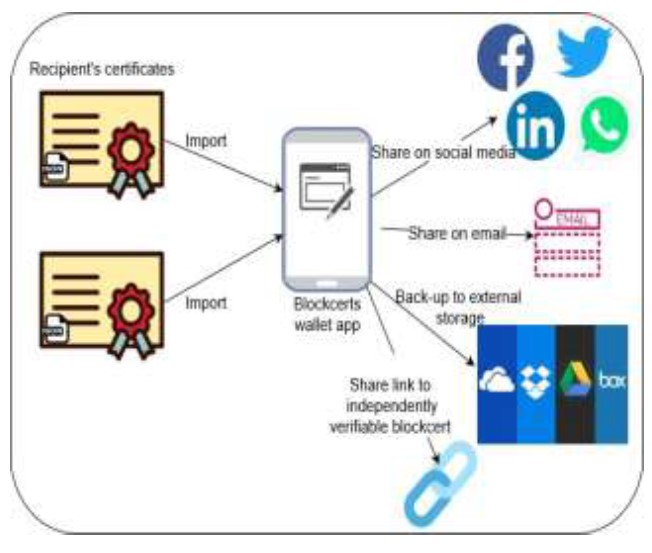
\includegraphics[width=\textwidth]{imgs/figure_2.8.1.jpg}
        \caption{Solution that will replace the conventional approach of birth/death certificate generation}
        \label{fig:Solution that will replace the conventional approach of birth/death certificate generation}
        \end{figure}
    \noindent{
       \underline{Results:}
       Our propose system provides integrity, privacy, transparency of certificate and anonymity of userIn this paper, we presented a solution that will replace the conventional approach of birth/death certificate generation. We have used blockchain technology and Blockcerts in the process of birth/death certification and validation. The solution includes registration of birth/death, creation of JSON file (digital certificate), public-private key cryptography to Achieve confidentiality using encryption and digital signature.


}
